\documentclass[aspectratio=169]{beamer}

% ── Theme & colours ──────────────────────────────────────────────────────────
\usetheme{Madrid}
\usecolortheme{default}
\definecolor{mainblue}{RGB}{30,70,130}
\definecolor{accentblue}{RGB}{70,130,200}
\definecolor{lightblue}{RGB}{220,235,250}
\definecolor{alertred}{RGB}{200,50,50}
\definecolor{compgreen}{RGB}{30,140,80}
\definecolor{damporange}{RGB}{210,100,20}

\setbeamercolor{frametitle}{bg=mainblue, fg=white}
\setbeamercolor{title}{fg=white}
\setbeamercolor{subtitle}{fg=lightblue}
\setbeamercolor{author}{fg=white}
\setbeamercolor{date}{fg=lightblue}
\setbeamercolor{palette primary}{bg=mainblue, fg=white}
\setbeamercolor{palette secondary}{bg=accentblue, fg=white}
\setbeamercolor{palette tertiary}{bg=mainblue, fg=white}
\setbeamercolor{block title}{bg=mainblue, fg=white}
\setbeamercolor{block body}{bg=lightblue, fg=black}
\setbeamercolor{structure}{fg=mainblue}

\usepackage{pifont}

% ── Packages ─────────────────────────────────────────────────────────────────
\usepackage{amsmath, amssymb, bm}
\usepackage{graphicx}
\usepackage{tikz}
\usetikzlibrary{shapes.geometric, arrows.meta, positioning, fit, backgrounds}
\usepackage{xcolor}
\usepackage{booktabs}
\usepackage{multicol}
\usepackage{tcolorbox}
\tcbuselibrary{skins, breakable}
\usepackage{multimedia}   % for \movie{}{}
\usepackage{hyperref}
% \usepackage{media9}
% \usepackage{animate}

% ── Custom boxes ─────────────────────────────────────────────────────────────
\tcbset{
  constraintbox/.style={
    enhanced, colback=lightblue, colframe=mainblue,
    fonttitle=\bfseries\small, coltitle=white,
    attach boxed title to top left={yshift=-2mm, xshift=4mm},
    boxed title style={colback=mainblue, sharp corners},
    arc=4pt, boxrule=1pt,
  }
}

\newcommand{\highlight}[2][yellow]{\colorbox{#1}{$\displaystyle #2$}}

% ── Meta ─────────────────────────────────────────────────────────────────────
\title{Deformable Linear Object Modeling \& State Estimation}
\author{Anders, Lauge and Mads}
\date{\today}

% ─────────────────────────────────────────────────────────────────────────────
\begin{document}

% ── Title slide ──────────────────────────────────────────────────────────────
\begin{frame}
  \titlepage
\end{frame}

% ═══════════════════════════════════════════════════════════════════════════
% 1. INTRODUCTION
% ═══════════════════════════════════════════════════════════════════════════
\begin{frame}{Introduction}
  \begin{columns}[T]

    \begin{column}{0.44\textwidth}
      \vspace{0.4em}
        Main objectives:
        \begin{itemize}
            \item Create accurate model of DLO, with real time capabilities 
            \item Use learning based methods to close gap between developed model and real life
            \item Combine models with existing vision based methods to do state estimation
        \end{itemize}
    \end{column}

    \begin{column}{0.52\textwidth}
      \begin{center}
        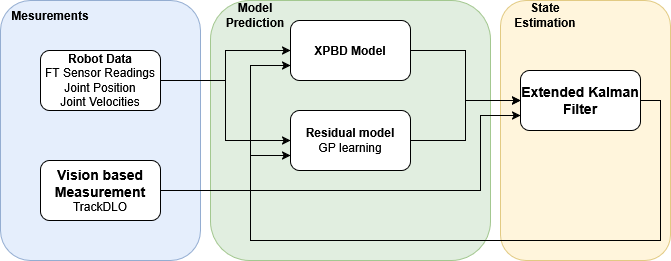
\includegraphics[width=\linewidth, keepaspectratio]{overview.png}
      \end{center}
    \end{column}

  \end{columns}
\end{frame}


% ═══════════════════════════════════════════════════════════════════════════
% 3. MODELING APPROACHES
% ═══════════════════════════════════════════════════════════════════════════
\begin{frame}{Modeling Approaches for DLOs}
  \begin{columns}[T]

    \begin{column}{0.31\textwidth}
      \begin{tcolorbox}[colback=lightblue!60, colframe=mainblue,
                        title={\small Mass-Spring System (MSS)},
                        fonttitle=\bfseries\small, coltitle=white,
                        arc=4pt, boxrule=0.8pt]
        \small
        \checkmark  \quad Simple to implement \\[4pt]
        \checkmark  \quad Fast to compute \\[4pt]
        \ding{55} \quad Lacks feasiblity with high flexibility \\[4pt]

      \end{tcolorbox}
    \end{column}

    \begin{column}{0.31\textwidth}
      \begin{tcolorbox}[colback=lightblue!60, colframe=mainblue,
                        title={\small Extended Pos.-Based Dynamics (XPBD)},
                        fonttitle=\bfseries\small, coltitle=white,
                        arc=4pt, boxrule=0.8pt]
        \small
        \checkmark  \quad Handles large deformations better \\[4pt]
        \checkmark  \quad Supports modeling of various objects\\[4pt]
        \checkmark  \quad Low computational cost \\[4pt]
        \ding{55}   \quad Physical fidelity is solver dependent\\[4pt]
      \end{tcolorbox}
    \end{column}

    \begin{column}{0.31\textwidth}
      \begin{tcolorbox}[colback=accentblue!25, colframe=gray!60,
                        title={\small Finite Element Analysis (FEM)},
                        fonttitle=\bfseries\small, coltitle=black,
                        arc=4pt, boxrule=1.2pt]
        \small
        \checkmark  \quad Very Accurate \\[4pt]
        \checkmark  \quad High Fidelity\\[4pt]
        \ding{55} \quad Complex to implement \\[4pt]
        \ding{55} \quad Not suited for Real time tasks \\[4pt]
      \end{tcolorbox}
    \end{column}

  \end{columns}

\end{frame}



% ═══════════════════════════════════════════════════════════════════════════
% 4. XPBD – HIGH-LEVEL OVERVIEW
% ═══════════════════════════════════════════════════════════════════════════
\begin{frame}{Extended Position Based Dynamics — Overview}
    For each timestep $dt$:
  \begin{center}
  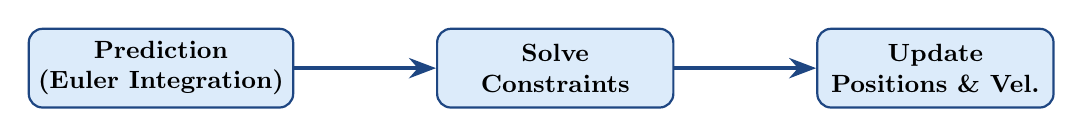
\begin{tikzpicture}[
      node distance=1.6cm,
      box/.style={draw=mainblue, fill=lightblue, rounded corners=5pt,
                  minimum width=3.0cm, minimum height=1.0cm,
                  align=center, font=\bfseries\small, thick},
      arrow/.style={-Stealth, thick, color=mainblue, line width=1.5pt},
  ]
    \node[box] (pred)  {Prediction\\(Euler Integration)};
    \node[box, right=1.8cm of pred]  (solve) {Solve\\Constraints};
    \node[box, right=1.8cm of solve] (upd)   {Update\\Positions \& Vel.};

    \draw[arrow] (pred)  -- (solve);
    \draw[arrow] (solve) -- (upd);

  \end{tikzpicture}
  \end{center}

  \vspace{0.5em}
  \begin{columns}[T]
    \begin{column}{0.32\textwidth}
      \begin{block}{1 — Prediction}
        Apply external forces (gravity) via explicit Euler to obtain \textit{predicted} positions and orientations.
      \end{block}
    \end{column}
    \begin{column}{0.32\textwidth}
      \begin{block}{2 — Constraint Solver}
        Constraints are iterativly solved $M_{iter}$ times in order to converge to correct position and orientation
      \end{block}
    \end{column}
    \begin{column}{0.32\textwidth}
      \begin{block}{3 — Velocity Update}
        Compute new velocities from the corrected positions.
      \end{block}
    \end{column}
  \end{columns}

  \vspace{0.6em}
  \small
  State vector per node: $\mathbf{x}_i = [\mathbf{p}_i,\, \mathbf{q}_i]^\top$
  with position $\mathbf{p}_i\in\mathbb{R}^3$ and orientation quaternion
  $\mathbf{q}_i\in\mathrm{SO}(3)$.
\end{frame}

% ═══════════════════════════════════════════════════════════════════════════
% 6. COSSERAT ROD THEORY
% ═══════════════════════════════════════════════════════════════════════════
\begin{frame}{Constraint Formulations : Cosserat Rod Theory}

  \begin{columns}[T]
    \begin{column}{0.52\textwidth}


      \vspace{0.8em}
      \textbf{Key assumptions:}
      \begin{itemize}
        \item Rod length $L \gg$ radius $r$ \;($L \gg r$)
        \item Described by a smooth centreline curve $r(s)$,\; $s\in[0,L]$
        \item Frame orientation captured by quaternion $q(s)$
      \end{itemize}

      \vspace{0.8em}
      \textbf{Deformation modes captured:}\\
      \begin{center}
      \small
      \begin{tabular}{ll}
        \toprule
        Mode & Strain measure\\
        \midrule
        Stretch / Shear & $\Gamma(s) = \frac{\partial r}{\partial s} - d_3(s)$\\[4pt]
        Bend / Twist    & $\Delta\Omega = \Omega - \Omega^0$\\
        \bottomrule
      \end{tabular}
      \end{center}
    \end{column}

    \begin{column}{0.44\textwidth}
      \begin{center}
        % Replace with your actual Cosserat rod figure
        \begin{tcolorbox}[colback=gray!10, colframe=gray!50,
                          arc=4pt, boxrule=0.8pt, halign=center]
          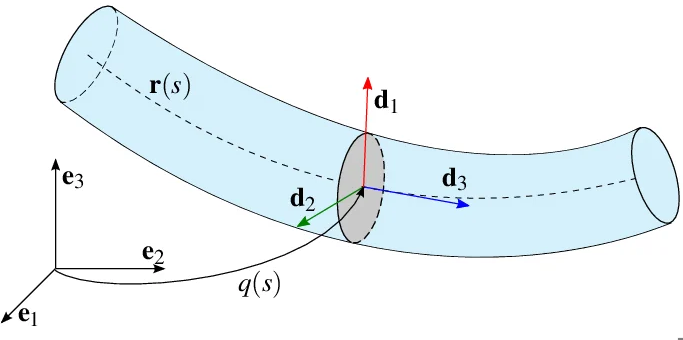
\includegraphics[width=0.85\linewidth]{cosserat.png}\\[1em]
          \small Directors $d_1, d_2, d_3$ defining the\\
          local material frame along the rod centreline and $e_1, e_2, e_3$ defines a fixed world frame.
        \end{tcolorbox}
      \end{center}
    \end{column}
  \end{columns}
\end{frame}

% ═══════════════════════════════════════════════════════════════════════════
% 7. CONSTRAINT FORMULATIONS
% ═══════════════════════════════════════════════════════════════════════════
\begin{frame}{Constraint Formulations : Cosserat Rod Theory}

  \begin{columns}[T]

    % ── Box 1: Stretch/Shear ────────────────────────────────────────────
    \begin{column}{0.32\textwidth}
      \begin{tcolorbox}[constraintbox, title={Stretch / Shear}]
        \small
        Between nodes $\mathbf{p}_1$, $\mathbf{p}_2$ with orientation $\mathbf{q}$:
        \begin{equation*}
          \mathbf{C}_s = \frac{\mathbf{p}_2 - \mathbf{p}_1}{l} - R(\mathbf{q})\,e_3
        \end{equation*}
        \vspace{2pt}
      \end{tcolorbox}
    \end{column}

    % ── Box 2: Bend/Twist ───────────────────────────────────────────────
    \begin{column}{0.32\textwidth}
      \begin{tcolorbox}[constraintbox, title={Bending / Twist}]
        \small
        Between adjacent orientations $\mathbf{q}$, $\mathbf{u}$:
        \begin{equation*}
          \mathbf{C}_b = \Im(\mathbf{q}^*\mathbf{u}) - s\,\Omega_0
        \end{equation*}
        \vspace{2pt}
       
      \end{tcolorbox}
    \end{column}

    % ── Box 3: TCP ──────────────────────────────────────────────────────
    \begin{column}{0.32\textwidth}
      \begin{tcolorbox}[constraintbox, title={Fixed Node to TCP}]
        \small
        Locks node 0 to end-effector (no slip):
        \begin{equation*}
          \mathbf{C}_\text{pos} = \mathbf{p}_0 - \mathbf{p}_\text{ee} = \mathbf{0}
        \end{equation*}
        \begin{equation*}
          \mathbf{C}_\text{ori} = \Im\!\left(\mathbf{q}_\text{ee}^*\,\mathbf{q}_i\right) = \mathbf{0}
        \end{equation*}
        \vspace{2pt}
      \end{tcolorbox}
    \end{column}
    

  \end{columns}
  \vspace{0.8em}
  \begin{tcolorbox}[colback=gray!10, colframe=gray!40, arc=3pt, boxrule=0.6pt]
    \small
    Note that analytical gradients can be obtained for each of these constraints, enabling fast computation of the Gauss-Seidel update
  \end{tcolorbox}
\end{frame}


% ═══════════════════════════════════════════════════════════════════════════
% 5. XPBD – KEY EQUATIONS
% ═══════════════════════════════════════════════════════════════════════════
\begin{frame}{XPBD — Position Correction \& Gauss-Seidel Update}

  \textbf{Position correction} (from linearised constraint):
  \begin{equation*}
    \Delta \mathbf{x} = \mathbf{W}\,\nabla \mathbf{C}(\mathbf{x})\,\Delta\lambda
    \qquad
    \mathbf{W} = \mathrm{diag}\!\left[m_1^{-1}\mathbf{I},\,\mathbf{I}_1^{-1},\;\ldots\right]
  \end{equation*}

  \vspace{0.3em}
  \textbf{Gauss-Seidel update} per constraint $j$:
  \begin{equation*}
    \Delta \lambda_j =
    \frac{
      -C_j(\mathbf{x})
      - \tilde{\alpha}_j\,\lambda_j
      - \gamma_j\bigl(C_j(\mathbf{x}) - C_j(\mathbf{x}^n)\bigr)
    }{
      (1+\gamma_j)\,\nabla C_j\,M^{-1}\nabla C_j^\top + \tilde{\alpha}_j
    }
  \end{equation*}

  \vspace{0.4em}
  \begin{columns}[T]
    \begin{column}{0.48\textwidth}
      \begin{tcolorbox}[colback=compgreen!15, colframe=compgreen,
                        title={Compliance $\tilde{\alpha}_j$},
                        fonttitle=\bfseries, coltitle=white,
                        arc=4pt, boxrule=1pt]
        \small
        $\tilde{\alpha}_j = \dfrac{\alpha_j}{\Delta t^2}$\\[4pt]
        $\alpha_j$ sets the \textbf{physical stiffness} of each constraint
        (bending, stretching, \ldots) — derived from material properties $E$, $G$.
      \end{tcolorbox}
    \end{column}
    \begin{column}{0.48\textwidth}
      \begin{tcolorbox}[colback=damporange!15, colframe=damporange,
                        title={Damping $\gamma_j$},
                        fonttitle=\bfseries, coltitle=white,
                        arc=4pt, boxrule=1pt]
        \small
        $\tilde{\beta}_j = \Delta t^2\,\beta_j,\quad
         \gamma_j = \dfrac{\alpha_j\beta_j}{\Delta t}$\\[4pt]
        $\beta_j$ is a \textbf{Rayleigh damping} coefficient — controls energy dissipation
      \end{tcolorbox}
    \end{column}
  \end{columns}

\end{frame}

\begin{frame}{Additional Modeling Work}

  \begin{columns}[T]

    \begin{column}{0.46\textwidth}
      \begin{block}{Contact Point Estimation}
        \begin{itemize}
          \item Detect where the DLO makes contact with its environment, based purely on FT sensor data and the XPBD model
          \item Enables more physically accurate simulation by incorporating contact
        \end{itemize}
      \end{block}
    \end{column}

    \begin{column}{0.46\textwidth}
      \begin{block}{Material Property Estimation}
        \begin{itemize}
          \item Estimate physical properties of the wire (stiffness, damping) from observations
          \item Allows the simulation to be tuned to match a real object
        \end{itemize}
      \end{block}
    \end{column}

  \end{columns}
\end{frame}

% ═══════════════════════════════════════════════════════════════════════════
% 8. EXTENDED KALMAN FILTER — MOTIVATION
% ═══════════════════════════════════════════════════════════════════════════
\begin{frame}{State Estimation: The Need for Filtering}

  \begin{columns}[T]
    \begin{column}{0.48\textwidth}
      \textbf{Problem:}
      \begin{itemize}
        \item XPBD model predicts wire motion, but is imperfect due to:
          \begin{itemize}
            \item Unmodeled forces and friction
            \item Uncertain material parameters
            \item Numerical discretization errors
          \end{itemize}
        \item Vision system (TrackDLO) provides noisy measurements of wire position
        \item Need \textit{fused} estimate combining both sources
      \end{itemize}
    \end{column}

    \begin{column}{0.48\textwidth}
      \begin{center}
        \begin{tcolorbox}[colback=lightblue!70, colframe=mainblue, arc=4pt, boxrule=1pt]
          \small\centering
          \textbf{Solution: Extended Kalman Filter}\\[6pt]
          Optimally blend model predictions with sensor measurements
        \end{tcolorbox}
      \end{center}
      \vspace{0.8em}
      \textbf{Key idea:}
      \begin{itemize}
        \item Predict state using physics model
        \item Correct using measurements
        \item Track uncertainty to weight each source
      \end{itemize}
    \end{column}
  \end{columns}

\end{frame}

% ═══════════════════════════════════════════════════════════════════════════
% 9. EXTENDED KALMAN FILTER — EQUATIONS
% ═══════════════════════════════════════════════════════════════════════════
\begin{frame}{Extended Kalman Filter — Two-Step Algorithm}

  \textbf{State vector:} $\mathbf{x} = [\mathbf{p}_1, \mathbf{v}_1, \mathbf{a}_1, \ldots, \mathbf{p}_n, \mathbf{v}_n, \mathbf{a}_n]^\top$ for $n$ nodes.

  \vspace{0.6em}
  \begin{columns}[T]

    \begin{column}{0.48\textwidth}
      \begin{tcolorbox}[colback=compgreen!15, colframe=compgreen,
                        title={Prediction Step},
                        fonttitle=\bfseries\small, coltitle=white,
                        arc=4pt, boxrule=1pt]
        \small
        Project state and covariance forward using kinematic model:
        \vspace{0.3em}
        \begin{align*}
          \hat{\mathbf{x}}^- &= f(\hat{\mathbf{x}}, \Delta t)\\
          \mathbf{P}^- &= \mathbf{F}\mathbf{P}\mathbf{F}^\top + \mathbf{Q}
        \end{align*}
        $\mathbf{F}$: state transition Jacobian\\
        $\mathbf{Q}$: process noise covariance
      \end{tcolorbox}
    \end{column}

    \begin{column}{0.48\textwidth}
      \begin{tcolorbox}[colback=damporange!15, colframe=damporange,
                        title={Update (Correction) Step},
                        fonttitle=\bfseries\small, coltitle=white,
                        arc=4pt, boxrule=1pt]
        \small
        Use measurement to correct the prediction:
        \vspace{0.3em}
        \begin{align*}
          \mathbf{K} &= \mathbf{P}^-\mathbf{H}^\top(\mathbf{H}\mathbf{P}^-\mathbf{H}^\top+\mathbf{R})^{-1}\\
          \hat{\mathbf{x}} &= \hat{\mathbf{x}}^- + \mathbf{K}(\mathbf{z} - \mathbf{H}\hat{\mathbf{x}}^-)\\
          \mathbf{P} &= (\mathbf{I} - \mathbf{K}\mathbf{H})\mathbf{P}^-
        \end{align*}
        $\mathbf{K}$: Kalman gain\\
        $\mathbf{R}$: measurement noise covariance\\
        $\hat{\mathbf{x}}$: Updated state estimate
      \end{tcolorbox}
    \end{column}

  \end{columns}

\end{frame}

% ═══════════════════════════════════════════════════════════════════════════
% 10. WIREEKF.PY — IMPLEMENTATION
% ═══════════════════════════════════════════════════════════════════════════
\begin{frame}{WireEKF.py — Implementation Details}

  \small
  \begin{columns}[T]
    \begin{column}{0.48\textwidth}
      \textbf{Core Components:}
      \begin{itemize}
        \item \textbf{State vector}: Position $\mathbf{p}$, velocity $\mathbf{v}$, acceleration $\mathbf{a}$ per node
        \item \textbf{Constant-acceleration model}: Kinematic prediction
          \begin{itemize}
            \item $\mathbf{p} \leftarrow \mathbf{p} + \mathbf{v}\Delta t + \frac{1}{2}\mathbf{a}\Delta t^2$
            \item $\mathbf{v} \leftarrow \mathbf{v} + \mathbf{a}\Delta t$
          \end{itemize}
        \item \textbf{XPBD callback}: Leverages physics model for prediction
        \item \textbf{Position-only measurement}: Vision system reports wire node positions
      \end{itemize}
    \end{column}

    \begin{column}{0.48\textwidth}
      \textbf{Tuning Parameters:}
      \begin{itemize}
        \item $\mathbf{Q}$: Controls trust in model
          \begin{itemize}
            \small
            \item High $Q$ $\Rightarrow$ filter relies more on measurements
            \item Low $Q$ $\Rightarrow$ filter trusts model predictions
          \end{itemize}
        \item $\mathbf{R}$: Controls trust in measurements
          \begin{itemize}
            \small
            \item High $R$ $\Rightarrow$ filter trusts model more
            \item Low $R$ $\Rightarrow$ filter trusts measurements more
          \end{itemize}
      \end{itemize}
      \vspace{0.4em}
      \begin{tcolorbox}[colback=alertred!15, colframe=alertred, arc=3pt, boxrule=0.8pt]
        \textbf{Key trade-off:} $Q/R$ ratio determines blend between model and measurements
      \end{tcolorbox}
    \end{column}
  \end{columns}

\end{frame}

% ═══════════════════════════════════════════════════════════════════════════
% 11. WHY EKF FOR WIRE TRACKING
% ═══════════════════════════════════════════════════════════════════════════
\begin{frame}{Why Extended Kalman Filter for Wire Tracking?}

  \begin{columns}[T]
    \begin{column}{0.48\textwidth}
      \textbf{Challenges in DLO State Estimation:}
      \begin{itemize}
        \item Model is only an approximation of reality
        \item Measurements are noisy and sparse (limited vision points)
        \item Wire dynamics are nonlinear (bending, gravity)
        \item Real-time constraints demand computational efficiency
      \end{itemize}
    \end{column}

    \begin{column}{0.48\textwidth}
      \textbf{EKF Advantages:}
      \begin{itemize*}
        \item \checkmark \quad Handles \textbf{nonlinearity} via linearization
        \item \checkmark \quad \textbf{Fuses} heterogeneous sensor data\\
        \quad \quad optimally
        \item \checkmark \quad Provides \textbf{uncertainty estimates} ($\mathbf{P}$)
        \item \checkmark \quad Computationally \textbf{efficient} for real-time
        \item \checkmark \quad \textbf{Adaptive}: Q/R tune trust in model vs.\ sensors
      \end{itemize*}
    \end{column}
  \end{columns}

  \vspace{0.8em}
  \begin{tcolorbox}[colback=compgreen!15, colframe=compgreen, arc=4pt, boxrule=1pt]
    \small
    \textbf{Result:} Better state estimates than either model or sensors alone. Essential for accurate robot control when fitting the end of a wire into a hole.
  \end{tcolorbox}

\end{frame}

% ═══════════════════════════════════════════════════════════════════════════
% 12. CURRENT VALIDATION & FUTURE INTEGRATION
% ═══════════════════════════════════════════════════════════════════════════
\begin{frame}{EKF Validation: Animation Output}

  \begin{columns}[T]
    \begin{column}{0.48\textwidth}
      \textbf{Current Stage (Simulation):}
      \begin{itemize}
        \item Validating EKF with synthetic data
        \item Wire suspended from fixed point, affected by gravity
        \item Simulink model provides synthetic measurements
        \item Tuning Q/R ratios to verify filter behavior
      \end{itemize}

      \vspace{0.8em}
      \textbf{Next Phase (Real Hardware):}
      \begin{itemize}
        \item Replace Simulink data with \textbf{TrackDLO} real-time tracking
        \item TrackDLO: Vision-based system detecting DLO node positions
        \item Plug TrackDLO output directly as measurements into EKF
        \item Validate state estimates during actual robot manipulation
      \end{itemize}
    \end{column}

    \begin{column}{0.48\textwidth}
      \centering
      \vspace{0.5em}
      \textbf{EKF Output Visualization}
      \begin{figure}
          \centering
          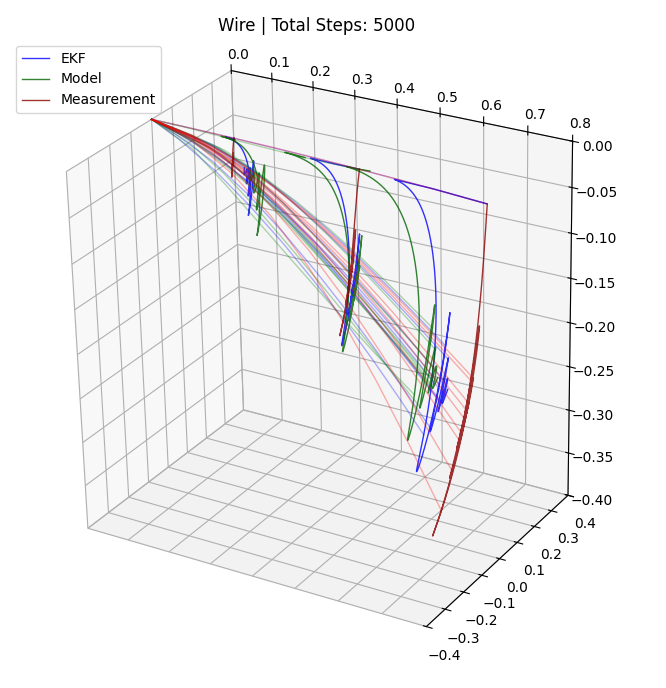
\includegraphics[width=1\linewidth]{EKF_5000.png}
      \end{figure}
    \end{column}
  \end{columns}
\end{frame}

\end{document}